\documentclass[12pt]{article}
\usepackage[margin=1in]{geometry}
\usepackage{amsmath}
\usepackage{amssymb}
\usepackage{fancyhdr}
\usepackage{pgfplots}
\usepackage{graphicx}
\usepackage{enumitem}
\usepackage{hyperref} 
\pgfplotsset{compat=1.16}


\author{Zhijie Xia, Yuan Liu, Zixing Wei, G-69}
\title{CPSC 471 Final Report}


\pagestyle{fancy}
\renewcommand{\headrulewidth}{0pt}
\renewcommand{\footrulewidth}{0pt}


\fancyhf{}
\rhead{
    Final Report
}
\rfoot{
    Page \thepage
}

\begin{document}
\maketitle
\newpage

\textbf{Abstract:}

\vspace*{5mm}
“YourStore” is a non-profit online shopping platform. Aside from its non-profit nature, its functionality is very similar to a retailer’s online shopping website, for example, Best Buy and its bestbuy.ca. It provides small stores a website application that is easy to configure and maintain.
The store owners will be given the permission to list other products, change the inventory, and track all the placed orders. All end users’ data (products, orders, inventories) will be stored in the database that can be accessed and modified when needed. The project’s core concept is providing an opportunity to store owners to sell their
products online, which is realized by a series of core functions, such as customers’ order placement, local stores’ order acceptance and arrange delivery . Order status is also updated at different stages of the order and tracked by all end-users.
Our project has similar functionalities to other commercial online shopping services. It facilitates a complete process of shopping order, realized by many core functions, such as customers’ order placement, sellers’ order acceptance and shipment. Order status is also updated at different stages of the order and tracked by all end-users. All CRUD (create, read, update and delete) functions can be realized via Postman, and our mobile-friendly web app can also visualize the entire user-flow from registration to order complete.
“YourStore” is made with React framework, Redux, Node.js, MongoDB, Express. With Node.js MongoDB, and Express, we were able to develop back-end API in javascript language to implement all necessary CRUD functions, as well as connect our back-end API to a mobile-friendly front-end web app, which is developed with a combination of React, Redux, Bootstrap. All API endpoints are properly connected to our database.


\newpage
\textbf{Introduction:}
\vspace*{5mm}

Since the prolonged pandemic has forced people to increasingly move their works and life online, many small sized 
local stores are suffering a plummeting in the number of in store shoppers. Thus, they desire to seize the opportunity to develop online businesses like other large-chain retail stores. This problem is partially solved by online workshops like Amazon, Ebay, and StockX. 
Their business model allows business owners to sell other products on their website by charging a substantial percentage of commission. Since the pandemic has lasted for a long time and there is no sign of an end at present, many local small-sized store owners argue the current business model that they build on the online platforms becomes less economically viable and not commercially sustainable for them when a considerable part of their revenue is being taken by the platform provider.

\vspace*{10mm}

\textbf{Our System:}
\vspace*{5mm}

"YourStore" is a non-profit online shopping platform. Aside from its non-profit nature, its functionality is very similar to a retailer’s online shopping website, for example, Best Buy and its bestbuy.ca. It provides small stores a website 
application that is easy to configure and maintain. The store owners will be given the permission to list other products, change the inventory, and track all the placed orders. All end users, data (products, orders, inventories) will be stored 
in the database that can be accessed and modified when needed. The project’s core concept is providing an opportunity to store owners to sell their products online, which is realized by a series of core functions, such as customers' order placement, local stores' 
order acceptance and arrange delivery . Order status is also updated at different stages of the order and tracked by all end-users.

\newpage 
\textbf{Project Design Description:}










\newpage 
\textbf{Project Design EER:}

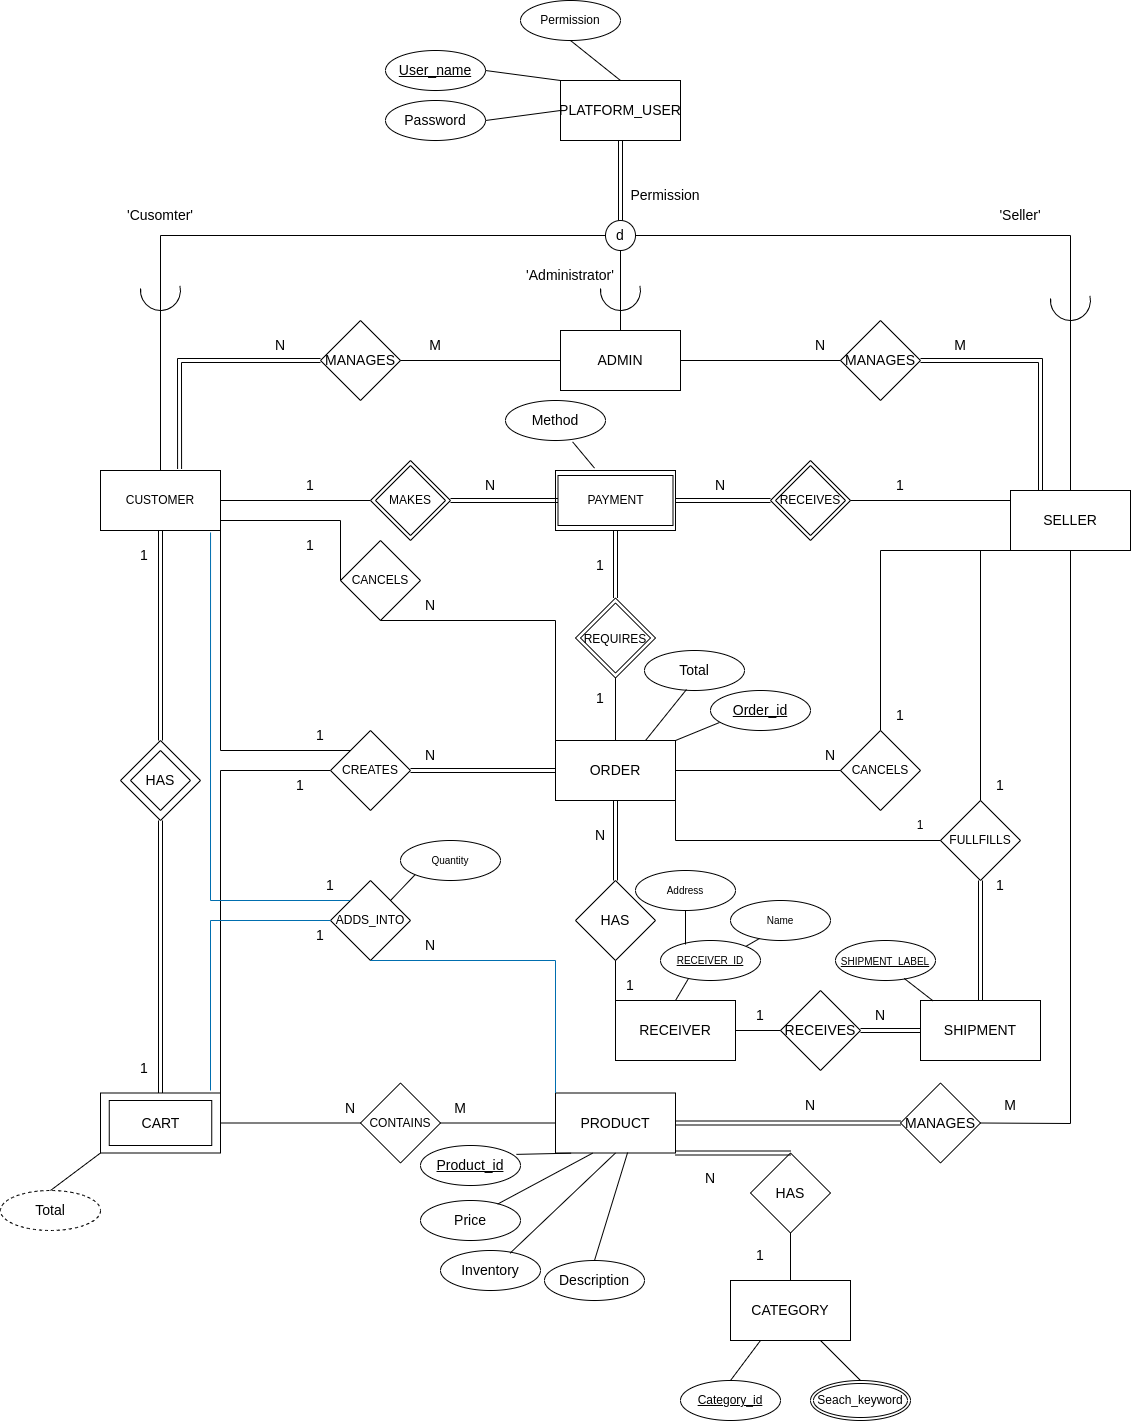
\includegraphics[height=.80\textheight]{Diagrams/onlineShopping_revised.png}

\newpage
\textbf{Implementation RMD:}
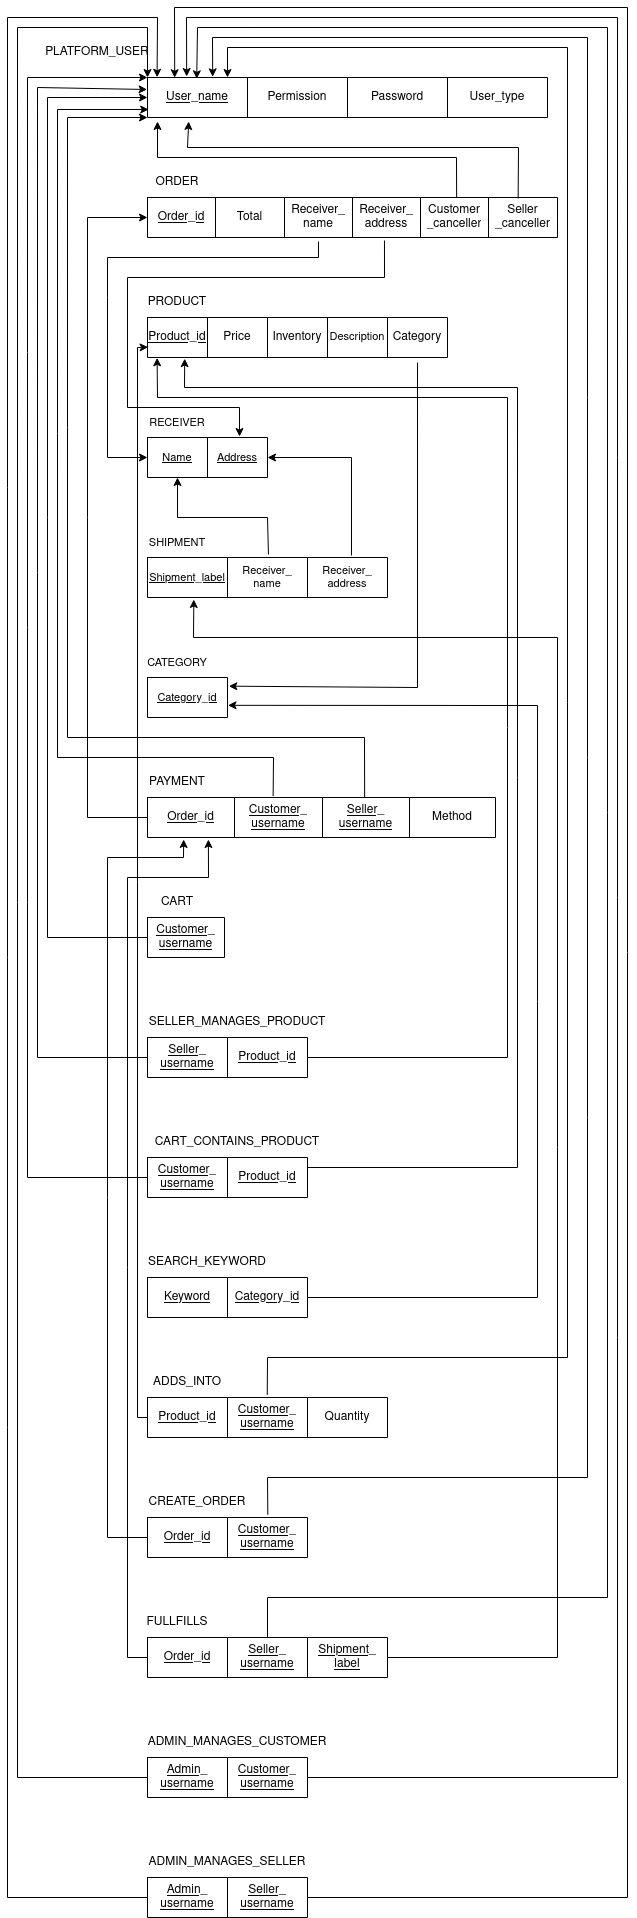
\includegraphics[height=.98\textheight]{Diagrams/relation.png}

\newpage 
\textbf{Implementation DBMS:}


\newpage

\textbf{Postman Docuementation:}

\begin{center}
    https://documenter.getpostman.com/view/20517678/Uyr4LftC
\end{center}

\newpage 
\textbf{User Guide:}


\end{document}